\documentclass[tikz, border=10pt]{standalone}
\usetikzlibrary{shapes, arrows.meta, positioning, calc}

\begin{document}
	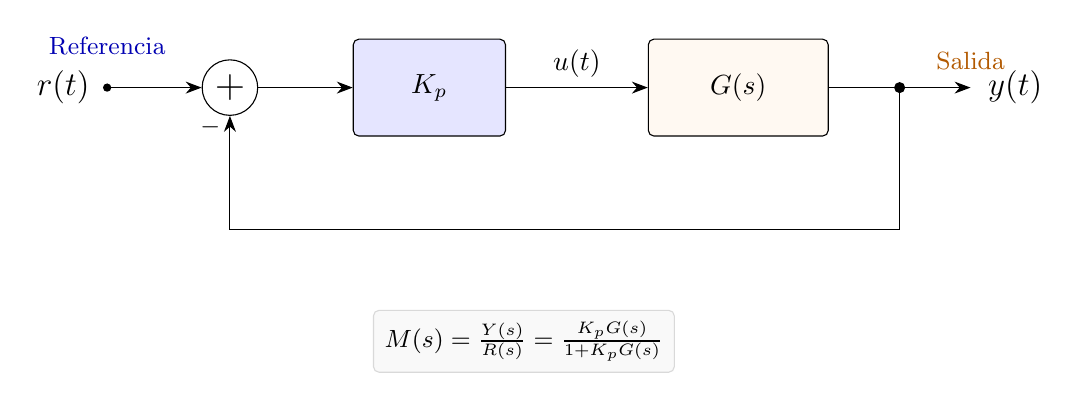
\begin{tikzpicture}[
		% Estilos unificados para mantener la consistencia visual de la memoria
		block/.style = {draw, fill=blue!10, rectangle, minimum height=3.5em, minimum width=5.5em, align=center, rounded corners=2pt},
		proc_block/.style = {draw, fill=orange!5, rectangle, minimum height=3.5em, minimum width=6.5em, align=center, rounded corners=2pt},
		sum/.style = {draw, fill=white, circle, inner sep=2pt},
		input/.style = {coordinate},
		output/.style = {coordinate},
		node distance=2.5cm,
		>={Stealth[scale=1.2]}
		]
		
		% --- EJE PRINCIPAL ---
		% Entrada (Referencia r)
		\node [input] (r_in) {};
		\node [left=0.1cm of r_in] {\large $r(t)$};
		
		% Sumador (+ / -)
		\node [sum, right=1.2cm of r_in] (sum) {\Large +};
		
		% Controlador Proporcional (K_p)
		\node [block, right=1.2cm of sum] (ctrl) {$K_p$};
		
		% Planta del motor/carro (G(s))
		\node [proc_block, right=1.8cm of ctrl] (plant) {$G(s)$};
		
		% Salida (y)
		\node [output, right=1.8cm of plant] (salida) {};
		\node [right=0.1cm of salida] {\large $y(t)$};
		
		% --- CONEXIONES ---
		\draw [->] (r_in) -- (sum);
		\draw [->] (sum) -- (ctrl);
		\draw [->] (ctrl) -- node[above] {$u(t)$} (plant);
		\draw [->] (plant) -- (salida);
		
		% Punto de ramificación para la realimentación unitaria de salida
		\coordinate (branch) at ($(plant.east) + (0.9,0)$);
		\fill (branch) circle (2pt);
		
		% Conexión de realimentación unitaria (H(s) = 1)
		\draw [->] (branch) -- ++(0,-1.8) -| node[left, pos=0.95] {\small $-$} (sum);
		
		% --- ANOTACIONES DE ADQUISICIÓN DE DATOS ---
		% Puntos de captura para el System Identification
		\fill (r_in) circle (1.5pt);
		\node [above=0.3cm of r_in, font=\small\color{blue!70!black}, align=center] {Referencia};
		
		\node [above=0.1cm of salida, font=\small\color{orange!70!black}, align=center] {Salida};
		
		% Texto explicativo inferior del bucle cerrado global M(s)
		\node [below=2.2cm of ctrl, xshift=1.2cm, font=\small\itshape, fill=gray!5, draw=gray!30, inner sep=4pt, rounded corners=2pt] 
		{$M(s) = \frac{Y(s)}{R(s)} = \frac{K_p G(s)}{1 + K_p G(s)}$};
		
	\end{tikzpicture}
\end{document}